\documentclass{article}

% PUDM @ NeurIPS 2026. Camera-ready version.
% Tiny Paper: at most 4 main pages. References, checklist, and
% appendix are unlimited. Extra figures live in the appendix.
\usepackage[final,dblblindworkshop]{neurips_2026}
\usepackage[utf8]{inputenc}
\usepackage[T1]{fontenc}
\usepackage{hyperref}
\hypersetup{hidelinks,pdfauthor={Shishun Dai},
  pdftitle={When Does RLVR Teach Physical Strategy? Measuring Simulator-Only Post-Training for CNC Planning}}
\usepackage{url}
\usepackage{booktabs}
\usepackage{amsfonts}
\usepackage{amsmath}
\usepackage{nicefrac}
\usepackage{microtype}
\usepackage{xcolor}
\usepackage{graphicx}
\usepackage{multirow}
\usepackage{tikz}
\usetikzlibrary{arrows.meta,positioning}

\newcommand{\validmetric}{\texttt{valid}}
\newcommand{\successmetric}{\texttt{success}}
\newcommand{\passk}{\mathrm{pass}@k}
\newcommand{\passat}[1]{\mathrm{pass}@#1}

% Reserved figure slot. Replace the box with a generated PDF/PNG;
% keep the caption, which already states the intended claim.
\newcommand{\figslot}[2]{%
  \fbox{\parbox[c][#1][c]{0.97\linewidth}{\centering\small\color{black!55}#2}}}

\title{When Does RLVR Teach Physical Strategy?\\
Measuring Simulator-Only Post-Training\\for CNC Planning}
\workshoptitle{Physical Understanding for Decision-Making}

% Camera-ready author information supplied by the author.
\author{%
  Shishun Dai \\
  Harvard University
}

\begin{document}
\maketitle

\begin{abstract}
We present a single-run case study of reinforcement learning from
verifiable rewards (RLVR) for CNC process planning, separating program
executability, strict machining success, and plan structure. Qwen3-8B
writes complete multi-setup G-code; an interpreter and voxel process
model supply the only post-SFT training feedback. The verifier is
audited with 166 checks and a separate 2.5D stock checker. Two exams
probe strategies described in the prompt but absent from teacher
trajectories: multi-tool roughing/finishing of one feature and regrouping
nonadjacent same-face features. GRPO improves modeled path validity
($86.0\!\to\!93.0\%$ IID; $59.0\!\to\!76.0\%$ on the setup exam)
and mean verifier reward ($-0.417\!\to\!-0.344$ validation).
Strict success changes by only $0.5$ percentage points on validation
and IID; both exams remain at $0/100$ with zero positive strategy
proxies. Individual repairs coexist with regressions. These results
describe one seed and a short, non-thinking training regime; they do
not distinguish limited exploration, SFT-induced behavior, generation
length, and reward or credit-assignment effects. The contribution is
an audited benchmark and a measured separation of outcomes, rather
than general conditions for strategy acquisition. We release the
frozen benchmark, verifier, and archived outputs for offline regrading.
\end{abstract}

\section{Introduction}
\label{sec:intro}

Foundation and world models increasingly support
decision-making~\citep{ha2018worldmodels,hafner2023dreamerv3,yang2024unisim,bruce2024genie,hu2023gaia1},
but predictive fidelity alone does not establish reliable action.  An
agent can still gouge a part or collide on a rapid.  It can also waste
setups.  We operationalize one aspect of physical understanding as
choosing actions that respect stock geometry and tool-machine
constraints.  We ask when post-training against a
physical grader adds process strategy beyond the demonstrations.

RLVR has improved language models where a checker can replace
preference
labels~\citep{lambert2024tulu3,guo2025deepseekr1,shao2024deepseekmath}.
The same recipe is now applied to physical
constraints~\citep{ji2025grounded}.  A reward can raise pass@1 while
sharpening support the base policy already
had~\citep{yue2025rlcapacity,yuan2026diversity}, so a gain on the
grader is not, by itself, new strategy.

We measure the split on CNC process planning, where every cut
irreversibly changes the stock.  The input is a semantic feature list
on fixed AL6061 stock, not STEP or drawings.  The policy
emits one multi-setup G-code document.  An interpreter and voxel stock
model grade interpreter acceptance, modeled path validity, and material state
(Figure~\ref{fig:system}).  Collision and tool reach are checked
explicitly.  We audit the grade with planted resolution films.  A
separate 2.5D engine and a 166-check battery provide further checks.

The teacher is deliberately local.  It uses one tool per feature and
preserves feature-list setup order.  It therefore never demonstrates
two strategies the grader can reward.  One is multi-tool roughing and
finishing.  The other reorders nonadjacent same-face features into one setup.  Both
rules are stated in the system prompt, but the teacher does not
implement them.  A $K{=}16$ parameter search can
reduce overload on a small multi-tool subset, but it cannot produce
either demonstration-absent composition (Appendix~\ref{app:extra}).
Closest work on G-code and CAD uses executable checks or formal
proofs~\citep{abdelaal2025gllm,lee2026correct,mallis2026cadtests}.  We
report greedy SFT and simulator-only
GRPO~\citep{shao2024deepseekmath,liu2025drgrpo}.  Two four-sample SFT
controls provide context.  They are any-of-four $\passat{4}$ and
reward-selected search-4.

Any-of-four $\passat{4}$ measures whether four SFT samples expose a
successful output; search-4 tests whether the coarse verifier selects
one.  Neither establishes that an unobserved behavior has zero
probability under SFT.  On both exams, both controls remain at $0/100$.
GRPO improves path validity and mean reward, while exam success and
strategy proxies remain zero. Occasional in-distribution repairs occur
(Figure~\ref{fig:paired}), but they are not representative.
Code, data, and archived outputs are available at
\url{https://github.com/pqori/CNC-RLVR}.

\begin{figure}[t]
  \centering
  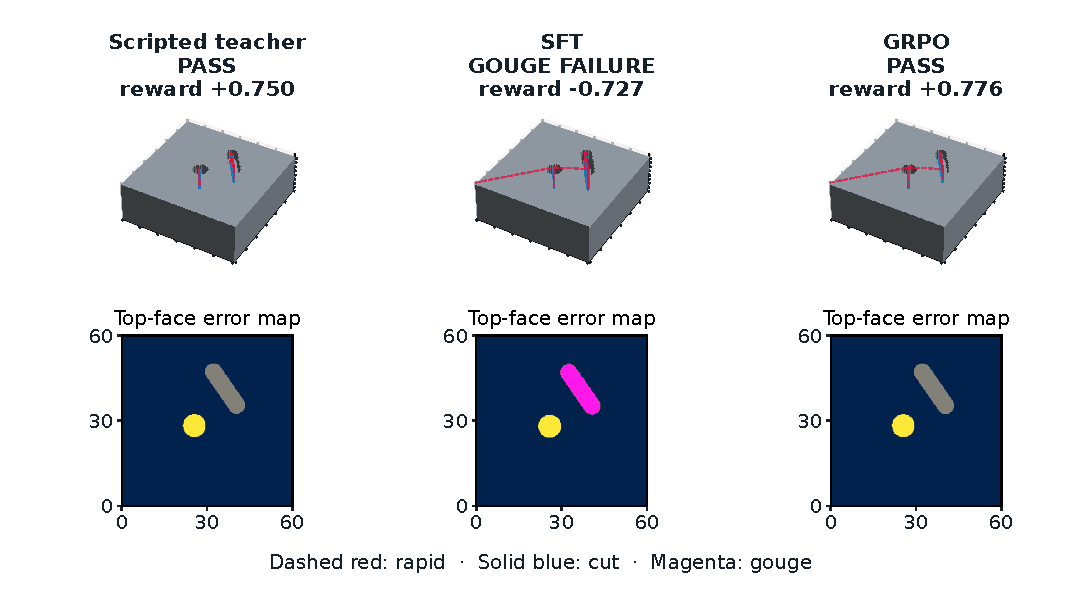
\includegraphics[width=\linewidth]{figures/local_repair.pdf}
  \caption{A rare local repair, not the mean effect.  On validation
  seed 5177, the top row shows commanded toolpaths (rapids dashed);
  the bottom row projects removed thickness (dark blue: zero; gray:
  intermediate; yellow: greater removal), with red for required material
  remaining and magenta for protected material removed. Maps use
  $0.2$\,mm voxels; policy verdicts and rewards use the audit-plus-spot
  protocol. SFT gouges; GRPO repairs this part. Aggregate success moves only
  $18.0\%\!\to\!18.5\%$ (Table~\ref{tab:policy}).}
  \label{fig:paired}
\end{figure}

\begin{figure}[t]
  \centering
  \footnotesize
  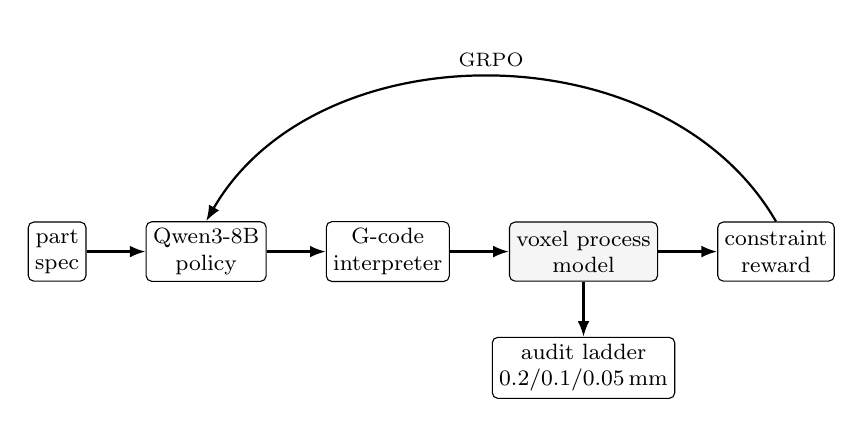
\begin{tikzpicture}[
    node distance=5.5mm and 7.5mm,
    box/.style={draw, rounded corners=2pt, align=center,
      minimum height=7.5mm, inner sep=2.5pt, font=\footnotesize},
    sim/.style={box, fill=black!4},
    flow/.style={-{Latex[length=2mm]}, thick},
  ]
    \node[box] (spec) {part\\spec};
    \node[box, right=of spec] (policy) {Qwen3-8B\\policy};
    \node[box, right=of policy] (interp) {G-code\\interpreter};
    \node[sim, right=of interp] (sim) {voxel process\\model};
    \node[box, right=of sim] (reward) {constraint\\reward};
    \node[box, below=7mm of sim] (audit) {audit ladder\\0.2/0.1/0.05\,mm};

    \draw[flow] (spec) -- (policy);
    \draw[flow] (policy) -- (interp);
    \draw[flow] (interp) -- (sim);
    \draw[flow] (sim) -- (reward);
    \draw[flow] (sim) -- (audit);
    \draw[flow] (reward.north) to[out=120,in=60]
      node[above, font=\scriptsize] {GRPO} (policy.north);
  \end{tikzpicture}
  \caption{Product spec to G-code document to interpreter and voxel
  process model.  GRPO uses the $0.2$\,mm grade with triggered
  $0.05$\,mm frontier checks; evaluation independently applies the
  fixed $0.1$\,mm audit and rechecks every audit-clean output at
  $0.05$\,mm.}
  \label{fig:system}
\end{figure}

\section{Task and verifier design}
\label{sec:method}

\paragraph{Task.}
Stock is $60\times60\times20$\,mm AL6061.  Milled features and drilled
holes may occur on any face.  The input is face-local feature
geometry. The policy emits a complete document without intermediate
simulator feedback, using a documented G-code subset
(Appendix~\ref{app:gcode}).  It uses absolute metric coordinates and
inline setup declarations.  Core commands control tools and motion.
The \verb+M3+ command starts the spindle.  Spindle speed and feed are fixed by the selected
tool and move geometry, not emitted by the policy.  Words outside the
dialect and unsupported modal state fail with a line number.

\paragraph{Grade.}
Every move is swept through a $0.2$\,mm voxel stock model.  Path
validity requires accepted syntax and modeled motion with no rapid or
holder collision. Removing protected material outside the tolerance envelope
is a gouge.  Tool reach and modeled load receive continuous severity
scores.  Ramp angle does too.  Any violation fails the corresponding
safety gate, although simulation continues to provide partial credit.
We report
\[
  \validmetric = \text{all safety gates pass}, \qquad
  \successmetric = \validmetric \wedge c\geq0.98
                    \wedge L_\infty\leq0.1\text{ mm},
\]
where $c$ is required-volume clearance and $L_\infty$ is worst residual
height.  Evaluation repeats the sweep at $0.1$\,mm.  Every audit-clean
output is then rechecked at $0.05$\,mm.
Appendix~\ref{app:verifier} gives the full objective and
severity terms.  Appendix~\ref{app:audit} reports 98 exact cross-engine
matches and a $166/166$ audit battery.

\paragraph{Designed demonstration gaps.}
The freeze has 1,999 teacher examples.  Validation and IID evaluation
each contain 200 parts.  Each exam contains 100.  The teacher uses one tool per feature
and feature-list setup order.  The multi-tool exam rewards using a
large mill to rough and a slender mill to finish tight corners; the
teacher's single-tool schedule overloads on every case.  The setup exam
interleaves three orientations; grouping by face reduces five setups
to three.  Local parameter search can reduce the multi-tool teacher's
overload, but cannot compose roughing and finishing tools.  On the
setup exam it recovers only $0.003$ of the reference's $0.202$ reward gain
(Appendix~\ref{app:extra}).  Modeled load is not exact geometry, so the
multi-tool axis is an auxiliary composition instrument; depth and tool
selection also change.

\section{Training and evaluation}
\label{sec:training}

We fine-tune Qwen3-8B~\citep{yang2025qwen3} for two epochs on the
teacher corpus with LoRA~\citep{hu2022lora}.  That SFT policy is the
imitation baseline and the GRPO start.  GRPO samples four documents per
prompt and uses group-relative advantages without further
demonstrations.  Each update uses eight prompts with four samples per
prompt. Fresh GRPO tasks come from the training generator, with neither
exam family explicitly mixed in. The run uses one seed with thinking
disabled. GRPO caps outputs at $8{,}192$ tokens; the released evaluation
configuration permits $24{,}576$ (Appendix~\ref{app:full}).
Coarse-clean, faster-than-reference rollouts are regraded at
$0.05$\,mm.  From four samples of the same SFT checkpoint, we report
both any-of-four $\passat{4}$ and search-4, which selects the highest
$0.2$\,mm reward.  These are test-time controls
(Appendix~\ref{app:full}).
Headline numbers are greedy.  Checkpoint selection is on validation
(step 50 of 100).

\section{Results}
\label{sec:results}

\paragraph{SFT baseline.}
SFT is path-valid on $88.5\%$ of validation and $86.0\%$ of IID
parts.  Strict success is only $36/200$ and $30/200$, respectively
(Appendix~\ref{app:extra}).  Both exams remain at $0/100$, with neither
strategy proxy observed.

\paragraph{GRPO changes path validity and reward more than strict success.}
Table~\ref{tab:policy} shows higher path validity on every split and
higher in-distribution reward.  Paired reward also improves when both
outputs are already path-valid.  The changes are $+0.066$ on validation
and $+0.044$ on IID, so transitions into path validity do not explain
the full gain.  Strict success changes by one part on each
in-distribution split.  Repairs are nearly balanced by regressions
(Appendix~\ref{app:paired}). Raw gouge counts also rise; unconditional
counts do not establish a higher conditional gouging rate. Neither
greedy GRPO nor either four-sample control achieves exam success or a
positive exam proxy. Figure~\ref{fig:paired} is therefore
a local repair, not the aggregate result.

\begin{table}[t]
  \caption{SFT greedy versus GRPO greedy at the validation-selected
  checkpoint (step 50).  Path-valid excludes hard path failures.
  Reward and success use the audit-plus-spot protocol.  Two-mill is a
  setup-level proxy, not feature attribution.}
  \label{tab:policy}
  \centering
  \small
  \begin{tabular}{llrr}
    \toprule
    split & metric & SFT greedy & GRPO greedy\\
    \midrule
    validation ($n{=}200$)
      & path-valid\% & 88.5 & 91.5\\
      & reward & $-0.417$ & $-0.344$\\
      & success\% & 18.0 & 18.5\\
      & gouge / $n$ & 105 & 112\\
      & two-mill\% & 7.0 & 7.0\\
    \midrule
    IID test ($n{=}200$)
      & path-valid\% & 86.0 & 93.0\\
      & reward & $-0.403$ & $-0.339$\\
      & success\% & 15.0 & 15.5\\
      & gouge / $n$ & 92 & 101\\
      & two-mill\% & 3.5 & 9.0\\
    \midrule
    OOT multi-tool ($n{=}100$)
      & path-valid\% & 89.0 & 96.0\\
      & reward & $-0.908$ & $-0.906$\\
      & success\% & 0.0 & 0.0\\
      & two-mill\% & 0.0 & 0.0\\
    \midrule
    OOT setups ($n{=}100$)
      & path-valid\% & 59.0 & 76.0\\
      & reward & $-0.906$ & $-0.884$\\
      & success\% & 0.0 & 0.0\\
      & G-code fails & 21 & 10\\
      & fewer-setups\% & 0.0 & 0.0\\
    \bottomrule
  \end{tabular}
\end{table}

\section{Discussion}
\label{sec:discussion}

The result separates three outcomes. GRPO produces more path-valid
programs and raises verifier reward, including among pairs already
path-valid under both policies. Strict part success changes little,
and raw gouge counts rise. A higher scalar grade therefore does not
by itself establish acquisition of a planning strategy.

Both probes require coordinated decisions across a long document.
Multi-tool machining links tool choices within a feature; setup grouping
requires nonlocal ordering. Terminal reward gives no direct attribution
to either decision. Although the verifier accepts scripted references,
the observed zeros cannot distinguish limited sampling support, SFT
suppression, the generation cap, reward scaling, or credit assignment.
The strategies are prompted, so these are tests of elicitation and
composition rather than discovery of an unstated rule.

The evidence is conditional on one validation-selected checkpoint from
one training seed. Reported differences are descriptive, and neither
zero exam success nor four unsuccessful samples establishes absent
policy support. The two-mill proxy can count tools serving different
features, while the setup proxy is gated on feasibility. Base-model,
larger-sample, reasoning-enabled, length-controlled, and additional-seed
comparisons remain unrun (Appendix~\ref{app:full}). Evaluation should
therefore report physical outcomes and inspect plan structure alongside
reward. The model's physical scope is stated in Appendix~\ref{app:compute}.

\clearpage
\bibliographystyle{plainnat}
\bibliography{references}

\appendix

\section{Additional tables and figures}
\label{app:extra}

\begin{table}[ht]
  \caption{Scripted baselines ($n{=}20$ per exam axis; parameter search
  uses a five-task subset).  Search can reduce overload without
  composing the demonstration-absent strategy.  These are not trained-policy
  results.}
  \label{tab:scripted}
  \centering
  \small
  \begin{tabular}{llrr}
    \toprule
    axis & plan & outcome & reward\\
    \midrule
    multi-tool & teacher & 0/20 & $0.308$\\
    multi-tool & geometry search ($K{=}16$) & 5/5 feasible & $0.515$\\
    multi-tool & two-tool reference & 20/20 & $0.750$\\
    \midrule
    setups & teacher (5 setups) & 20/20 & $0.650$\\
    setups & parameter search ($K{=}16$) & 5/5 & $0.653$\\
    setups & grouped reference (3 setups) & 20/20 & $0.852$\\
    \bottomrule
  \end{tabular}
\end{table}

\begin{table}[ht]
  \caption{Greedy SFT on the frozen splits.  ``Final'' applies the
  audit-plus-spot protocol.  \validmetric{} means all safety gates
  pass.  Path-valid rates are higher ($88.5\%$ / $86.0\%$ IID-family).}
  \label{tab:main}
  \centering
  \small
  \begin{tabular}{lrrrr}
    \toprule
    split & \validmetric\% & success@0.2 & success final & reward\\
    \midrule
    validation & 35.5 & 20.0 & 18.0 & $-0.417$\\
    IID test & 39.5 & 18.0 & 15.0 & $-0.403$\\
    OOT multi-tool & 0.0 & 0.0 & 0.0 & $-0.908$\\
    OOT setups & 1.0 & 0.0 & 0.0 & $-0.906$\\
    \bottomrule
  \end{tabular}
\end{table}

\paragraph{Paired diagnostics.}
\label{app:paired}
Validation contains two SFT-failure to GRPO-success repairs and one
regression.  IID contains three repairs and two regressions.  Among
pairs that are path-valid under both policies, mean reward changes by
$+0.066$ on validation and $+0.044$ on IID.
The two-mill proxy requires two distinct mills to remove stock in one
setup. They may serve different features, so the IID increase from
$3.5\%$ to $9.0\%$ does not establish same-feature roughing/finishing.
The fewer-setups proxy requires a feasible program with a lower
setup count than its teacher; unsuccessful regrouping attempts can
therefore be missed. Neither proxy alone establishes strategy completion.

\begin{figure}[t]
  \centering
  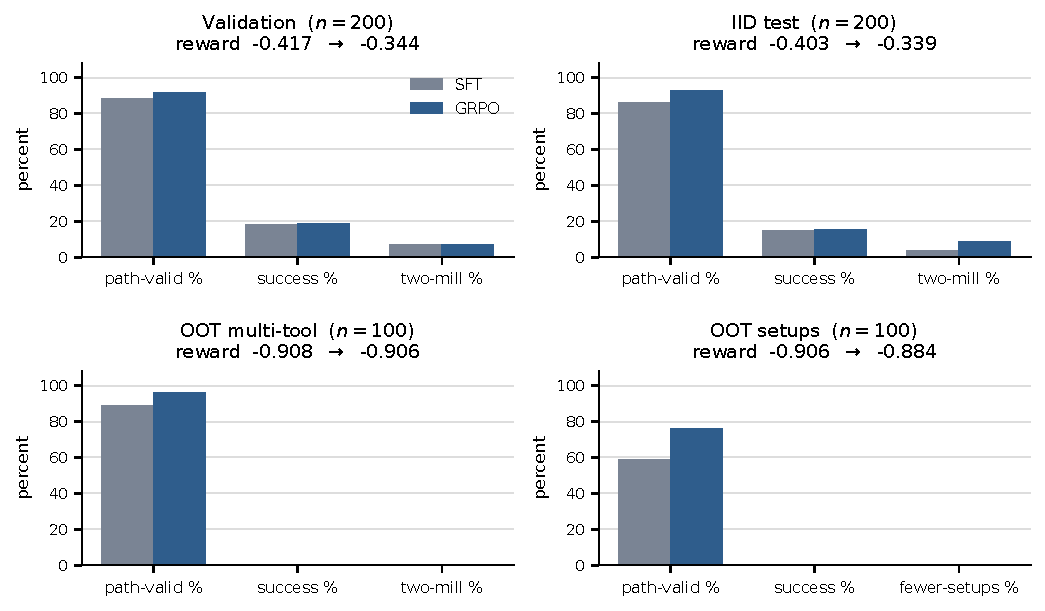
\includegraphics[width=\linewidth]{figures/score_move.pdf}
  \caption{Where the process-model score moves.  Path validity and reward
  improve. Success changes little; exam proxies remain zero. Two-mill
  means two mills cut in one setup; it is not the multi-tool exam
  name.  Numbers are Table~\ref{tab:policy}.}
  \label{fig:metrics}
\end{figure}

\begin{figure}[t]
  \centering
  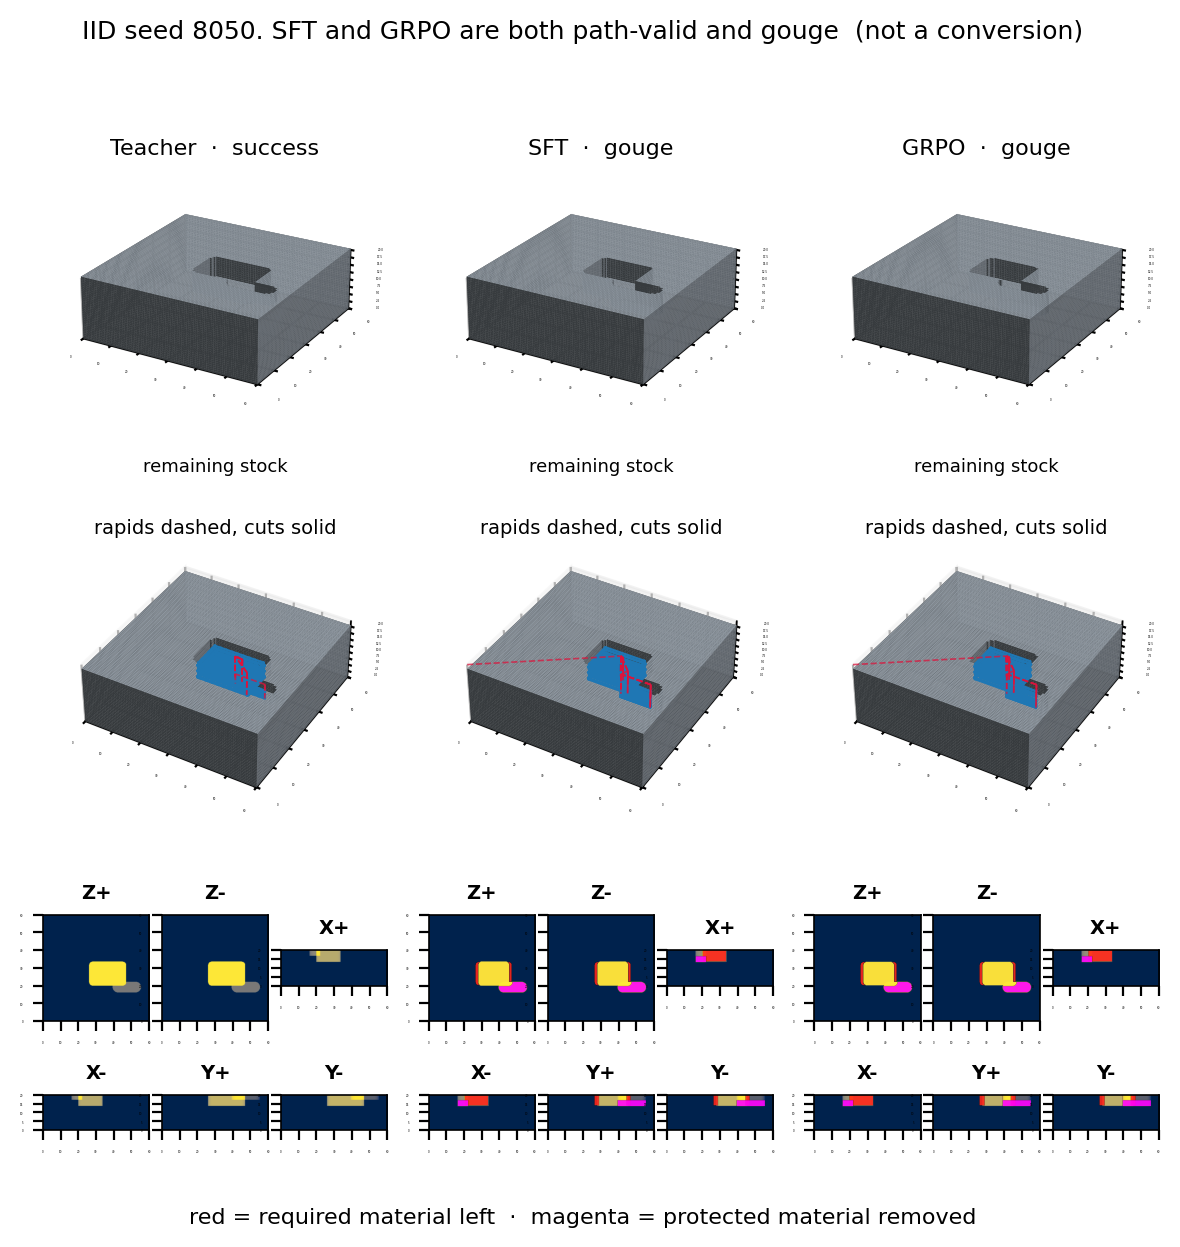
\includegraphics[width=\linewidth]{figures/typical_iid.png}
  \caption{Typical in-distribution programs (IID seed 8050).  SFT and
  GRPO are both path-valid and both gouge.  Leftover is red; gouge is magenta.}
  \label{fig:beforeafter}
\end{figure}

\begin{figure}[t]
  \centering
  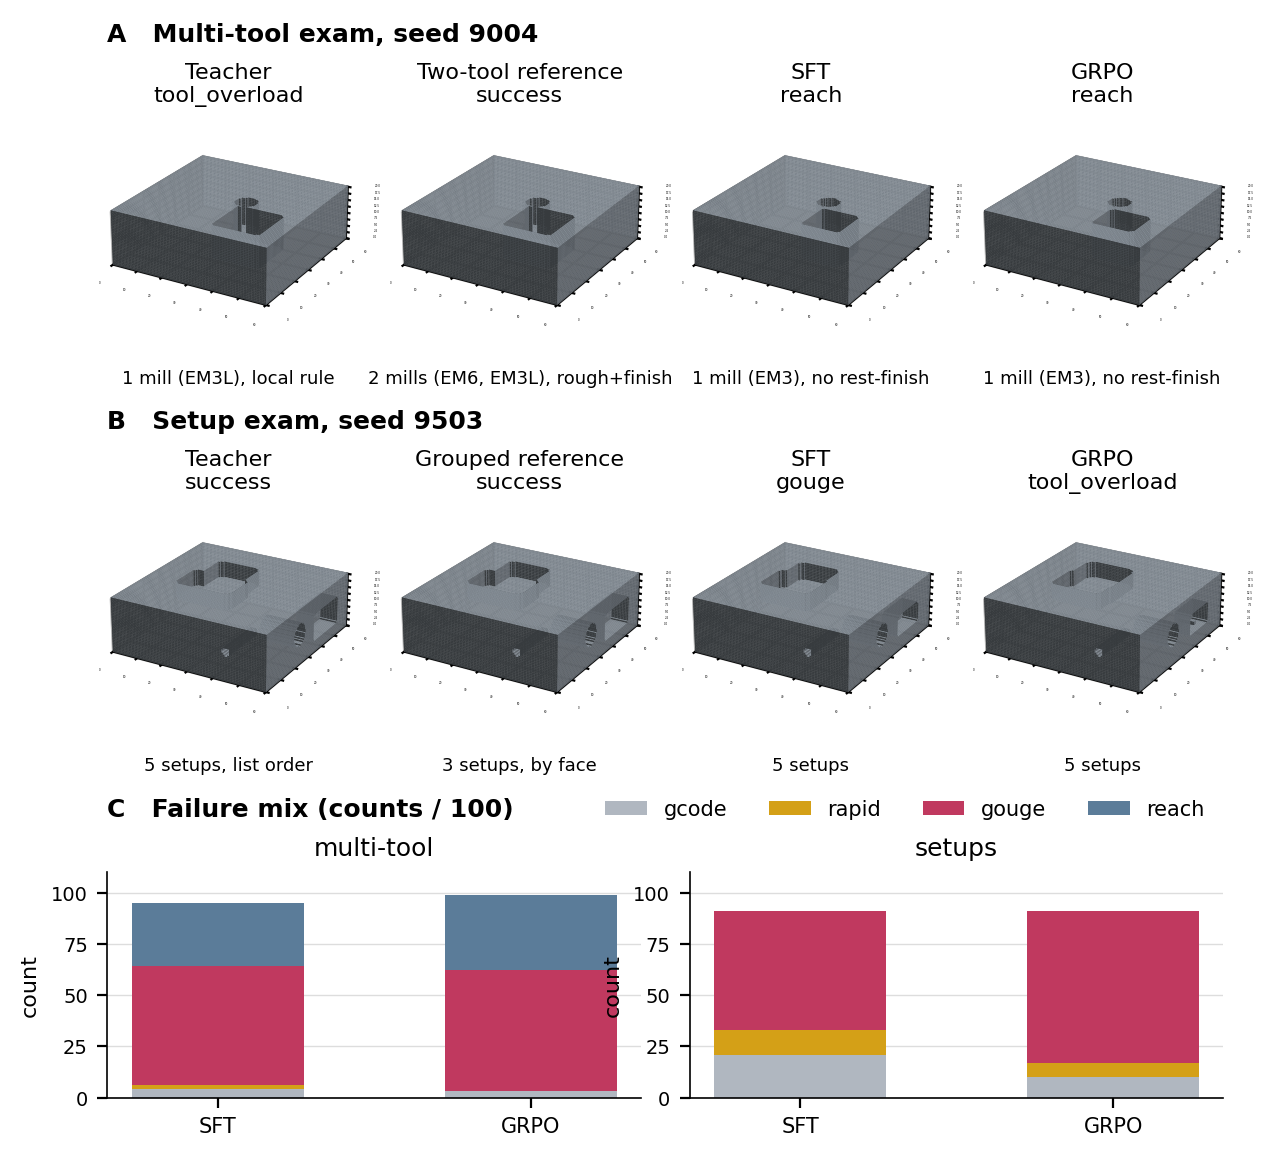
\includegraphics[width=\linewidth]{figures/exam_strategy.png}
  \caption{The exams ask for a different plan.  Panel A shows seed
  9004.  The teacher overloads one long mill, while the two-tool
  reference succeeds.  SFT and GRPO still use one mill.  Panel B shows
  seed 9503.  Grouping cuts five setups to three, while both policies
  keep five.  Panel C shows the failure mix.}
  \label{fig:exams}
\end{figure}

\section{Full task and G-code dialect}
\label{app:gcode}

\paragraph{Coordinate frames.}
Features use face-local $(u,v)$ coordinates in the frame seen by the tool
after reorientation.  A setup declaration selects one of six
axis-aligned faces.  The $X,Y$ coordinates are face-local.  The entered
stock face defines $Z=0$, with negative $Z$ inside the material.  One
interpreter therefore handles both side and top machining.

\paragraph{Dialect.}
A document begins with \verb+G21 G90+.  The \verb+(SETUP F)+ directive
opens a setup, while \verb+T<n> M6+ changes tools.  The spindle starts
with \verb+M3+.  Linear motion uses \verb+G0+ or \verb+G1+.
\verb+G2+ and \verb+G3+ express I/J-offset arcs.  Equal endpoints denote
a full circle, while a $Z$ word creates a helix.  Coordinates are modal.
RPM and feed are injected.  The document ends with \verb+M30+.
Unsupported controller features are rejected.  These include cutter
compensation and canned cycles.  Incremental coordinates and R-form arcs
are also rejected.  Unknown words fail with a line number.  Drills cut
only axially.  Endmills may ramp or helix but may not plunge.

\begin{small}
\begin{verbatim}
G21 G90
(SETUP Z+)
T8 M6
M3
G0 X18.000 Y22.000 Z2.000
G3 X20.400 Y22.000 Z-1.050 I1.200 J0.000
G3 I-1.200 J0.000 Z-2.100
G1 X24.000
G0 Z2.000
M30
\end{verbatim}
\end{small}

\paragraph{Fixed cutting schedule.}
Material is fixed to AL6061.  Each tool has one canonical spindle
speed/feed pair.  Descending mill entries use half feed, while flat
cuts use full feed.
\begin{center}
\begin{tabular}{lrr@{\qquad}lrr}
\toprule
tool & rpm & feed & tool & rpm & feed\\
\midrule
EM3/EM3L & 29,178 & 1,400.5 & EM6 & 14,589 & 2,100.8\\
EM10 & 8,754 & 2,101.0 & EM12 & 7,295 & 2,801.3\\
D3 & 9,549 & 458.4 & D5/D8 & 5,730/3,581 & 458.4\\
\bottomrule
\end{tabular}
\end{center}
Feeds are in mm/min.  The interpreter injects these values from tool
choice.

\section{Verifier implementation and objective}
\label{app:verifier}

\paragraph{Voxel sweep.}
The training engine stores a $300\times300\times100$ byte grid at
$0.2$\,mm resolution.  Each normalized motion primitive is sampled with
an error-bounded chord spacing; only a localized neighborhood of voxels is
tested and subtracted.  Required-removal and must-keep masks are generated
independently from feature geometry.  Side operations require a true 3D
state.  A cross-hole can create solid--air--solid columns that a single
heightfield cannot represent.

\paragraph{Geometric and controller checks.}
Controller checks cover parsing and modal state.  They also enforce
coordinate bounds and setup limits.  Geometric checks detect rapid and
holder collisions.  They enforce face access and tool compatibility.
Entry geometry and completion are checked separately.  Teacher documents must
round-trip through emit--parse--emit byte-identically and produce identical
motion primitives and metrics.

\paragraph{Load model.}
The current code measures newly removed volume over one-second cutting
windows.  It computes $\mathrm{MRR}=V/t$, where $t$ is the union of newly
removed voxel-center contact intervals.  This excludes zero-removal recuts
and air-feed padding.  Equivalent G1 segmentation leaves the result
unchanged.  Cutting power is $P=k_c\mathrm{MRR}$.  Mean force is
$F=P/v_c$.  Endmill capacity uses a cantilever-deflection envelope.
Spindle power provides a second cap.  With
$u=\max(F/F_{\max},P/P_{\max})$, evaluation reports $u>1$ as load-unsafe
and never counts it correct.  Training continues the counterfactual path
after overload and grades the severity continuously.

\paragraph{Training reward.}
Reward v9 defines normalized ramp-slope utilization
$u_r=\tan(\theta_{\max})/\tan(5^\circ)$.  Evaluation requires $u_r\leq1$,
but, as with load, simulation continues after an excess so training retains
a severity signal.  The reward first computes
\[
\begin{aligned}
q={}&c-0.25\,\mathrm{clip}_{[0,3]}(t/t_{\rm ref})
       -0.60\,\mathbf 1[L_\infty>0.1]\\
    &-2\max(0,0.98-c)-0.05\min(s_{\rm excess},3)\\
    &-0.05\phi(u)-0.05\phi(u_r)-1.54\phi(u_{\rm reach})
     -0.06\phi(g),\\[2pt]
r={}&\begin{cases}
-1,&\text{path-invalid hard failure},\\
q,&q\geq-0.90,\\
-0.898769+0.001368q,&q<-0.90.
\end{cases}
\end{aligned}
\]
Here $t_{\rm ref}$ is the teacher cycle time when the teacher is
feasible.  The multi-tool reference supplies it otherwise.
The term $s_{\rm excess}$ counts setups beyond the number of required
feature faces.  Path-invalid failures include malformed controller
state and hard motion failures.  Rapid or holder collision is a hard
motion failure, as is illegal tool motion.
For $z=\max(0,(u-0.8)/0.2)$,
$\phi(u)=\min(20,z^2)$ for $z\leq1$, and
$\phi(u)=\min(20,2z-1)$ otherwise; $\phi(u_r)$ uses the identical
dimensionless shape.  Ramps through roughly $4^\circ$ are unpenalized.
The penalty is 0.05 at the $5^\circ$ limit and remains continuous above
it.  Pure vertical non-center-cutting plunges remain hard failures.  The
load coefficient is the smallest 0.05-grid value above a 10\% margin on
paired intervention calibration.  Safe candidates dominated unsafe
counterparts on 42/42 calibration tasks and 16/16 held-out tasks.  Half
strength passed 95.2\% and 93.8\%, respectively.
For flute utilization $u_{\rm reach}=d_{\max}/L_{\rm flute}$,
$\phi(u_{\rm reach})=\min(20,\max(0,u_{\rm reach}-1)/0.25)$, so every
use through the exact flute limit is penalty-free.  The calibrated reach
coefficient 1.54 achieved 270/270 calibration and 405/405 held-out
safe-plan dominance.  Half strength passed only 94.4\% of calibration pairs.
Gouge severity $g$ is the maximum physical penetration beyond the analytic
dimensional-tolerance envelope, with
$\phi(g)=\min(20,g/(0.1\,\mathrm{mm}))$. Coefficient 0.06 is the smallest
0.01-grid value above a 10\% margin on 1,160 paired calibration shortcuts
and achieved 576/576 dominance on disjoint held-out geometries.  Half
strength achieved 86.1\% and 94.1\%, respectively.
Tool wear is measured but excluded.  Evaluation preserves all four
modeled safety gates and reports their severities separately.
The path-valid raw objective is bounded below by $-37.46$, which maps to
$-0.95$; the canonical reference
remains $0.75$.  The strictly increasing map preserves every path-valid plan
ordering and leaves all rewards at or above $-0.90$ unchanged while
guaranteeing that any executable partial trajectory beats malformed output
at $-1$.

\section{Benchmark construction and reference ladder}
\label{app:benchmark}

Tasks are generated deterministically from integer seeds and regenerated
during evaluation to detect prompt or RNG drift.  Verified teacher pairs
are retained only if they pass the frozen checker.  The release contains
the following splits.
\begin{center}
\begin{tabular}{lrrl}
\toprule
split & tasks & teacher success & purpose\\
\midrule
train & 1,999 & 1,999 & SFT\\
validation & 200 & 200 & model selection\\
IID evaluation & 200 & 200 & interpolation\\
OOT multi-tool & 100 & 0 under frozen load & composition\\
OOT setups & 100 & 100 & sequencing\\
\bottomrule
\end{tabular}
\end{center}
All 1,999 teacher plans use one tool per feature.  In 541 plans, the
feature order makes the teacher revisit a face rather than regroup
nonadjacent same-face features.
The locked Qwen3 tokenizer measures a maximum teacher completion of
19,737 tokens across the frozen splits.  SHA-256 hashes cover every
JSONL file.  The reference ladder compares the teacher, a $K{=}16$
stepdown/stepover search that cannot alter strategy.  Hand-constructed
references provide the structural comparison.

\paragraph{Teacher-failure taxonomy.}
Failures first separate controller execution from physical outcomes.
Physical outcomes then distinguish geometry from process efficiency.
A gain limited to controller execution is not evidence of physical
strategy.

\section{Training details}
\label{app:full}

\paragraph{SFT.}
Qwen3-8B uses LoRA rank 64 with $\alpha=128$ on all linear layers.
Training uses learning rate $10^{-4}$ for two epochs.  Loss applies only
to completions.  Thinking mode is
disabled and prompt formatting is byte-identical across training and
evaluation. We retain the Qwen3 tokenizer and causal language-model
output head, with no CNC-specific tokens, vocabulary resizing, or
separate action head.

\paragraph{GRPO.}
For each prompt, $K{=}4$ documents receive
\[
A_i=r_i-\frac{1}{K}\sum_{j=1}^K r_j,
\]
without standard-deviation normalization.  The update uses rank-64
LoRA with clipping $\epsilon=0.2$.  The KL coefficient is $0.04$.
The learning rate is $10^{-5}$.  Each step uses eight prompts, and the
run lasts at most 100 steps.  Document decoding is unconstrained.
The $8{,}192$-token training cap is below the frozen $19{,}737$-token
teacher maximum.  Cap-truncated outputs are incomplete and receive the
parser-failure reward of $-1$.  The imposed cap can therefore confound
length with model capability. Evaluation permits $24{,}576$ output
tokens in the released configuration; the $8{,}192$ limit applies to
GRPO training. The teacher maximum does not establish a minimum
solution length or a truncation rate. Original generation token IDs,
stop reasons, and complete training rollouts are not included in the
release, so training-time truncation frequencies cannot be recovered
from the archived evaluation text. The run fixes
model/data RNG seeds and writes immutable metadata plus per-rollout
parse/path/load fields and coarse-versus-spot rewards.

\paragraph{Four-sample controls.}
SFT sampling uses temperature 1.0 with four candidates per task.
Any-of-four $\passat{4}$ records whether at least one candidate passes
the audit-plus-spot protocol.  Search-4 instead selects the candidate
with highest $0.2$\,mm reward.  Exact ties retain the first candidate.
Any-of-four reaches $18.0\%$ on validation and $16.5\%$ on IID.
Search-4 reaches $16.5\%$ and $15.0\%$, respectively.  Both controls
remain at $0\%$ on the exams.
The selected step-50 policy had seen about 1,600 rollouts.  The full
run generated about 3,200 and took 8,304 seconds on the eight-GPU node.

\paragraph{Interpretation and unrun controls.}
We did not run equal-total-rollout RAFT~\citep{dong2023raft} or a
pre-SFT base measurement. Larger-sample support analysis, thinking-enabled
or plan-then-code generation, operation-level advantages, and a
grammar-locked typed arm also remain unrun. The small group size and
short training budget can limit exploration of coordinated program
changes. The monotone reward-tail map preserves rankings but compresses
reward differences, which matters for unnormalized advantages; its
causal effect is untested. Additional seeds and controlled comparisons
are needed to separate these explanations. Their absence limits the
interpretation (Section~\ref{sec:discussion}).

\section{Audit battery and exploit protocol}
\label{app:audit}

The adversarial battery checks all coordinate frames and analytic
removal volumes.  It probes access failures and tool compatibility.
Separate tests cover geometric boundaries and reward attribution.
Load behavior and entry domains receive dedicated checks.  The final
group verifies document round trips and malformed-program rejection.
The submission receipt records 166 passing checks.  The separately
implemented 2.5D stock checker matches 98 applicable plan comparisons
exactly. It shares motion expansion and path discretization with the
voxel checker; these comparisons do not independently validate load,
all controller behavior, or multi-face execution.
Ten overloaded multi-tool teachers are excluded from that comparison.
Four overloaded manual side-face plans are also excluded.

\paragraph{Resolution aliasing.}
A legal $0.08$\,mm film passes all grids.  A $0.16$\,mm film is invisible
at the $0.2$\,mm training grid but fails at the routine $0.1$\,mm audit
and the $0.05$\,mm spot grid.  A near-spec construction can appear clean
on both fixed grids.  Randomized spot selection detects the planted case.

\paragraph{Volumetric and interpolation attacks.}
Clearance alone can hide tall thin residual slivers, so completion also
uses worst residual height.  Coarse arc chords can undercut corners.
Error-bounded sampling prevents denser sampling from buying reward.

\paragraph{Reward ordering and load padding.}
The valid objective's affine map reserves a strict margin above malformed
output.  Executable first-operation prefixes across 20 generated tasks test
this ordering.  Force-window MRR divides by the union of newly removed
voxel-center contact intervals.  Zero-removal recuts must leave measured
utilization unchanged.  Cleared prefixes and equivalent G1 segmentations
provide separate checks.

\paragraph{Post-training protocol.}
During GRPO, a $0.05$\,mm grade replaces the coarse reward when a
geometry-clean candidate is faster than its reference.  Final evaluation
grades every output at $0.2$ and $0.1$\,mm.  Every audit-clean candidate
is then rechecked at $0.05$\,mm.  Outputs that already fail at
$0.1$\,mm retain that reward and verdict.  Any new
discrepancy is minimized and assigned an exploit class.  It is then added
to the battery without reusing the affected split for selection.

\section{Compute and reproducibility}
\label{app:compute}

The public release is available at \url{https://github.com/pqori/CNC-RLVR}.
The measurement uses one AWS p5.48xlarge node with eight 80\,GB H100 GPUs.
SFT and GRPO both use one process per GPU; GRPO colocates vLLM with each
data-parallel policy replica.  The supplement includes the frozen Python
package lock and the benchmark hashes.  It also includes training code and
archived outputs.  Model checkpoints and complete wall-clock accounting
are not included.  Reproducing model generation therefore requires
rerunning SFT and GRPO.  The reported outputs can be regraded offline.

\paragraph{Physical scope.}
The checker omits fixture geometry and machine dynamics.  No machine
trials were conducted.  A passing grade does not authorize physical
execution.

\section{Author checklist}

\section*{NeurIPS Paper Checklist}

The checklist does not count toward the page limit.


\begin{enumerate}

\item {\bf Claims}
    \item[] Question: Do the main claims made in the abstract and introduction accurately reflect the paper's contributions and scope?
    \item[] Answer: \answerYes{}
    \item[] Justification: The abstract and Section~\ref{sec:intro} report a single-run comparison of modeled path validity, verifier reward, strict success, and exam proxies. Section~\ref{sec:discussion} limits interpretation to the evaluated training configuration.
    \item[] Guidelines:
    \begin{itemize}
        \item The answer \answerNA{} means that the abstract and introduction do not include the claims made in the paper.
        \item The abstract and/or introduction should clearly state the claims made, including the contributions made in the paper and important assumptions and limitations. A \answerNo{} or \answerNA{} answer to this question will not be perceived well by the reviewers.
        \item The claims made should match theoretical and experimental results, and reflect how much the results can be expected to generalize to other settings.
        \item It is fine to include aspirational goals as motivation as long as it is clear that these goals are not attained by the paper.
    \end{itemize}

\item {\bf Limitations}
    \item[] Question: Does the paper discuss the limitations of the work performed by the authors?
    \item[] Answer: \answerYes{}
    \item[] Justification: Section~\ref{sec:discussion} and Appendices~\ref{app:full} and~\ref{app:compute} discuss the single seed, training budget, distinct training and evaluation caps, missing controls, proxy limitations, and omitted machine physics.
    \item[] Guidelines:
    \begin{itemize}
        \item The answer \answerNA{} means that the paper has no limitation while the answer \answerNo{} means that the paper has limitations, but those are not discussed in the paper.
        \item The authors are encouraged to create a separate ``Limitations'' section in their paper.
        \item The paper should point out any strong assumptions and how robust the results are to violations of these assumptions (e.g., independence assumptions, noiseless settings, model well-specification, asymptotic approximations only holding locally). The authors should reflect on how these assumptions might be violated in practice and what the implications would be.
        \item The authors should reflect on the scope of the claims made, e.g., if the approach was only tested on a few datasets or with a few runs. In general, empirical results often depend on implicit assumptions, which should be articulated.
        \item The authors should reflect on the factors that influence the performance of the approach. For example, a facial recognition algorithm may perform poorly when image resolution is low or images are taken in low lighting. Or a speech-to-text system might not be used reliably to provide closed captions for online lectures because it fails to handle technical jargon.
        \item The authors should discuss the computational efficiency of the proposed algorithms and how they scale with dataset size.
        \item If applicable, the authors should discuss possible limitations of their approach to address problems of privacy and fairness.
        \item While the authors might fear that complete honesty about limitations might be used by reviewers as grounds for rejection, a worse outcome might be that reviewers discover limitations that aren't acknowledged in the paper. The authors should use their best judgment and recognize that individual actions in favor of transparency play an important role in developing norms that preserve the integrity of the community. Reviewers will be specifically instructed to not penalize honesty concerning limitations.
    \end{itemize}

\item {\bf Theory assumptions and proofs}
    \item[] Question: For each theoretical result, does the paper provide the full set of assumptions and a complete (and correct) proof?
    \item[] Answer: \answerNA{}
    \item[] Justification: The paper is an empirical measurement; it contains no theorems.
    \item[] Guidelines:
    \begin{itemize}
        \item The answer \answerNA{} means that the paper does not include theoretical results.
        \item All the theorems, formulas, and proofs in the paper should be numbered and cross-referenced.
        \item All assumptions should be clearly stated or referenced in the statement of any theorems.
        \item The proofs can either appear in the main paper or the supplemental material, but if they appear in the supplemental material, the authors are encouraged to provide a short proof sketch to provide intuition.
        \item Inversely, any informal proof provided in the core of the paper should be complemented by formal proofs provided in appendix or supplemental material.
        \item Theorems and Lemmas that the proof relies upon should be properly referenced.
    \end{itemize}

    \item {\bf Experimental result reproducibility}
    \item[] Question: Does the paper fully disclose all the information needed to reproduce the main experimental results of the paper to the extent that it affects the main claims and/or conclusions of the paper (regardless of whether the code and data are provided or not)?
    \item[] Answer: \answerYes{}
    \item[] Justification: Sections~\ref{sec:method}--\ref{sec:training} and Appendices~\ref{app:gcode}--\ref{app:full} specify the dialect, splits, reward, GRPO hyperparameters, and evaluation ladder.
    \item[] Guidelines:
    \begin{itemize}
        \item The answer \answerNA{} means that the paper does not include experiments.
        \item If the paper includes experiments, a \answerNo{} answer to this question will not be perceived well by the reviewers: Making the paper reproducible is important, regardless of whether the code and data are provided or not.
        \item If the contribution is a dataset and\slash or model, the authors should describe the steps taken to make their results reproducible or verifiable.
        \item Depending on the contribution, reproducibility can be accomplished in various ways. For example, if the contribution is a novel architecture, describing the architecture fully might suffice, or if the contribution is a specific model and empirical evaluation, it may be necessary to either make it possible for others to replicate the model with the same dataset, or provide access to the model. In general. releasing code and data is often one good way to accomplish this, but reproducibility can also be provided via detailed instructions for how to replicate the results, access to a hosted model (e.g., in the case of a large language model), releasing of a model checkpoint, or other means that are appropriate to the research performed.
        \item While NeurIPS does not require releasing code, the conference does require all submissions to provide some reasonable avenue for reproducibility, which may depend on the nature of the contribution. For example
        \begin{enumerate}
            \item If the contribution is primarily a new algorithm, the paper should make it clear how to reproduce that algorithm.
            \item If the contribution is primarily a new model architecture, the paper should describe the architecture clearly and fully.
            \item If the contribution is a new model (e.g., a large language model), then there should either be a way to access this model for reproducing the results or a way to reproduce the model (e.g., with an open-source dataset or instructions for how to construct the dataset).
            \item We recognize that reproducibility may be tricky in some cases, in which case authors are welcome to describe the particular way they provide for reproducibility. In the case of closed-source models, it may be that access to the model is limited in some way (e.g., to registered users), but it should be possible for other researchers to have some path to reproducing or verifying the results.
        \end{enumerate}
    \end{itemize}


\item {\bf Open access to data and code}
    \item[] Question: Does the paper provide open access to the data and code, with sufficient instructions to faithfully reproduce the main experimental results, as described in supplemental material?
    \item[] Answer: \answerYes{}
    \item[] Justification: The public repository includes the verifier and training code, frozen synthetic splits, archived outputs and summaries, audit receipts, checksums, and exact commands to reproduce the tables and rerun evaluation.
    \item[] Guidelines:
    \begin{itemize}
        \item The answer \answerNA{} means that paper does not include experiments requiring code.
        \item Please see the NeurIPS code and data submission guidelines (\url{https://neurips.cc/public/guides/CodeSubmissionPolicy}) for more details.
        \item While we encourage the release of code and data, we understand that this might not be possible, so \answerNo{} is an acceptable answer. Papers cannot be rejected simply for not including code, unless this is central to the contribution (e.g., for a new open-source benchmark).
        \item The instructions should contain the exact command and environment needed to run to reproduce the results. See the NeurIPS code and data submission guidelines (\url{https://neurips.cc/public/guides/CodeSubmissionPolicy}) for more details.
        \item The authors should provide instructions on data access and preparation, including how to access the raw data, preprocessed data, intermediate data, and generated data, etc.
        \item The authors should provide scripts to reproduce all experimental results for the new proposed method and baselines. If only a subset of experiments are reproducible, they should state which ones are omitted from the script and why.
        \item At submission time, to preserve anonymity, the authors should release anonymized versions (if applicable).
        \item Providing as much information as possible in supplemental material (appended to the paper) is recommended, but including URLs to data and code is permitted.
    \end{itemize}


\item {\bf Experimental setting/details}
    \item[] Question: Does the paper specify all the training and test details (e.g., data splits, hyperparameters, how they were chosen, type of optimizer) necessary to understand the results?
    \item[] Answer: \answerYes{}
    \item[] Justification: Split sizes, LoRA and GRPO settings, decoding budget, token cap, and checkpoint selection are in Sections~\ref{sec:method}--\ref{sec:training} and Appendix~\ref{app:full}.
    \item[] Guidelines:
    \begin{itemize}
        \item The answer \answerNA{} means that the paper does not include experiments.
        \item The experimental setting should be presented in the core of the paper to a level of detail that is necessary to appreciate the results and make sense of them.
        \item The full details can be provided either with the code, in appendix, or as supplemental material.
    \end{itemize}

\item {\bf Experiment statistical significance}
    \item[] Question: Does the paper report error bars suitably and correctly defined or other appropriate information about the statistical significance of the experiments?
    \item[] Answer: \answerNo{}
    \item[] Justification: Paired transition counts are reported, but no uncertainty intervals or significance tests are presented. The comparison uses one training seed and is interpreted descriptively.
    \item[] Guidelines:
    \begin{itemize}
        \item The answer \answerNA{} means that the paper does not include experiments.
        \item The authors should answer \answerYes{} if the results are accompanied by error bars, confidence intervals, or statistical significance tests, at least for the experiments that support the main claims of the paper.
        \item The factors of variability that the error bars are capturing should be clearly stated (for example, train/test split, initialization, random drawing of some parameter, or overall run with given experimental conditions).
        \item The method for calculating the error bars should be explained (closed form formula, call to a library function, bootstrap, etc.)
        \item The assumptions made should be given (e.g., Normally distributed errors).
        \item It should be clear whether the error bar is the standard deviation or the standard error of the mean.
        \item It is OK to report 1-sigma error bars, but one should state it. The authors should preferably report a 2-sigma error bar than state that they have a 96\% CI, if the hypothesis of Normality of errors is not verified.
        \item For asymmetric distributions, the authors should be careful not to show in tables or figures symmetric error bars that would yield results that are out of range (e.g., negative error rates).
        \item If error bars are reported in tables or plots, the authors should explain in the text how they were calculated and reference the corresponding figures or tables in the text.
    \end{itemize}

\item {\bf Experiments compute resources}
    \item[] Question: For each experiment, does the paper provide sufficient information on the computer resources (type of compute workers, memory, time of execution) needed to reproduce the experiments?
    \item[] Answer: \answerNo{}
    \item[] Justification: Appendix~\ref{app:compute} identifies the p5.48xlarge / 8$\times$H100 setup and rollout count, but wall-clock time for each training stage and total exploratory compute were not reconstructed.
    \item[] Guidelines:
    \begin{itemize}
        \item The answer \answerNA{} means that the paper does not include experiments.
        \item The paper should indicate the type of compute workers CPU or GPU, internal cluster, or cloud provider, including relevant memory and storage.
        \item The paper should provide the amount of compute required for each of the individual experimental runs as well as estimate the total compute.
        \item The paper should disclose whether the full research project required more compute than the experiments reported in the paper (e.g., preliminary or failed experiments that didn't make it into the paper).
    \end{itemize}

\item {\bf Code of ethics}
    \item[] Question: Does the research conducted in the paper conform, in every respect, with the NeurIPS Code of Ethics \url{https://neurips.cc/public/EthicsGuidelines}?
    \item[] Answer: \answerYes{}
    \item[] Justification: The study uses a simulated machining verifier and synthetic parts; no human subjects or scraped personal data.
    \item[] Guidelines:
    \begin{itemize}
        \item The answer \answerNA{} means that the authors have not reviewed the NeurIPS Code of Ethics.
        \item If the authors answer \answerNo, they should explain the special circumstances that require a deviation from the Code of Ethics.
        \item The authors should make sure to preserve anonymity (e.g., if there is a special consideration due to laws or regulations in their jurisdiction).
    \end{itemize}


\item {\bf Broader impacts}
    \item[] Question: Does the paper discuss both potential positive societal impacts and negative societal impacts of the work performed?
    \item[] Answer: \answerYes{}
    \item[] Justification: Appendix~\ref{app:compute} states that a simulated pass does not authorize physical execution. The intended benefit is inspectable evaluation before physical trials; misuse of simulated passes could damage parts or equipment.
    \item[] Guidelines:
    \begin{itemize}
        \item The answer \answerNA{} means that there is no societal impact of the work performed.
        \item If the authors answer \answerNA{} or \answerNo, they should explain why their work has no societal impact or why the paper does not address societal impact.
        \item Examples of negative societal impacts include potential malicious or unintended uses (e.g., disinformation, generating fake profiles, surveillance), fairness considerations (e.g., deployment of technologies that could make decisions that unfairly impact specific groups), privacy considerations, and security considerations.
        \item The conference expects that many papers will be foundational research and not tied to particular applications, let alone deployments. However, if there is a direct path to any negative applications, the authors should point it out. For example, it is legitimate to point out that an improvement in the quality of generative models could be used to generate Deepfakes for disinformation. On the other hand, it is not needed to point out that a generic algorithm for optimizing neural networks could enable people to train models that generate Deepfakes faster.
        \item The authors should consider possible harms that could arise when the technology is being used as intended and functioning correctly, harms that could arise when the technology is being used as intended but gives incorrect results, and harms following from (intentional or unintentional) misuse of the technology.
        \item If there are negative societal impacts, the authors could also discuss possible mitigation strategies (e.g., gated release of models, providing defenses in addition to attacks, mechanisms for monitoring misuse, mechanisms to monitor how a system learns from feedback over time, improving the efficiency and accessibility of ML).
    \end{itemize}

\item {\bf Safeguards}
    \item[] Question: Does the paper describe safeguards that have been put in place for responsible release of data or models that have a high risk for misuse (e.g., pre-trained language models, image generators, or scraped datasets)?
    \item[] Answer: \answerNA{}
    \item[] Justification: The work fine-tunes a public 8B model on synthetic CNC tasks; it does not release a dual-use generator or scraped dataset.
    \item[] Guidelines:
    \begin{itemize}
        \item The answer \answerNA{} means that the paper poses no such risks.
        \item Released models that have a high risk for misuse or dual-use should be released with necessary safeguards to allow for controlled use of the model, for example by requiring that users adhere to usage guidelines or restrictions to access the model or implementing safety filters.
        \item Datasets that have been scraped from the Internet could pose safety risks. The authors should describe how they avoided releasing unsafe images.
        \item We recognize that providing effective safeguards is challenging, and many papers do not require this, but we encourage authors to take this into account and make a best faith effort.
    \end{itemize}

\item {\bf Licenses for existing assets}
    \item[] Question: Are the creators or original owners of assets (e.g., code, data, models), used in the paper, properly credited and are the license and terms of use explicitly mentioned and properly respected?
    \item[] Answer: \answerYes{}
    \item[] Justification: Qwen3-8B is cited~\citep{yang2025qwen3}; the public README links its Apache-2.0 license, does not redistribute its weights, and identifies the upstream licenses of required libraries.
    \item[] Guidelines:
    \begin{itemize}
        \item The answer \answerNA{} means that the paper does not use existing assets.
        \item The authors should cite the original paper that produced the code package or dataset.
        \item The authors should state which version of the asset is used and, if possible, include a URL.
        \item The name of the license (e.g., CC-BY 4.0) should be included for each asset.
        \item For scraped data from a particular source (e.g., website), the copyright and terms of service of that source should be provided.
        \item If assets are released, the license, copyright information, and terms of use in the package should be provided. For popular datasets, \url{paperswithcode.com/datasets} has curated licenses for some datasets. Their licensing guide can help determine the license of a dataset.
        \item For existing datasets that are re-packaged, both the original license and the license of the derived asset (if it has changed) should be provided.
        \item If this information is not available online, the authors are encouraged to reach out to the asset's creators.
    \end{itemize}

\item {\bf New assets}
    \item[] Question: Are new assets introduced in the paper well documented and is the documentation provided alongside the assets?
    \item[] Answer: \answerYes{}
    \item[] Justification: The public repository documents the synthetic benchmark, dialect, verifier, split purposes, evaluation protocol, archived outputs, limitations, safety scope, checksums, and reproduction commands.
    \item[] Guidelines:
    \begin{itemize}
        \item The answer \answerNA{} means that the paper does not release new assets.
        \item Researchers should communicate the details of the dataset\slash code\slash model as part of their submissions via structured templates. This includes details about training, license, limitations, etc.
        \item The paper should discuss whether and how consent was obtained from people whose asset is used.
        \item At submission time, remember to anonymize your assets (if applicable). You can either create an anonymized URL or include an anonymized zip file.
    \end{itemize}

\item {\bf Crowdsourcing and research with human subjects}
    \item[] Question: For crowdsourcing experiments and research with human subjects, does the paper include the full text of instructions given to participants and screenshots, if applicable, as well as details about compensation (if any)?
    \item[] Answer: \answerNA{}
    \item[] Justification: No crowdsourcing or human-subjects research.
    \item[] Guidelines:
    \begin{itemize}
        \item The answer \answerNA{} means that the paper does not involve crowdsourcing nor research with human subjects.
        \item Including this information in the supplemental material is fine, but if the main contribution of the paper involves human subjects, then as much detail as possible should be included in the main paper.
        \item According to the NeurIPS Code of Ethics, workers involved in data collection, curation, or other labor should be paid at least the minimum wage in the country of the data collector.
    \end{itemize}

\item {\bf Institutional review board (IRB) approvals or equivalent for research with human subjects}
    \item[] Question: Does the paper describe potential risks incurred by study participants, whether such risks were disclosed to the subjects, and whether Institutional Review Board (IRB) approvals (or an equivalent approval/review based on the requirements of your country or institution) were obtained?
    \item[] Answer: \answerNA{}
    \item[] Justification: No human-subjects research.
    \item[] Guidelines:
    \begin{itemize}
        \item The answer \answerNA{} means that the paper does not involve crowdsourcing nor research with human subjects.
        \item Depending on the country in which research is conducted, IRB approval (or equivalent) may be required for any human subjects research. If you obtained IRB approval, you should clearly state this in the paper.
        \item We recognize that the procedures for this may vary significantly between institutions and locations, and we expect authors to adhere to the NeurIPS Code of Ethics and the guidelines for their institution.
        \item For initial submissions, do not include any information that would break anonymity (if applicable), such as the institution conducting the review.
    \end{itemize}

\item {\bf Declaration of LLM usage}
    \item[] Question: Does the paper describe the usage of LLMs if it is an important, original, or non-standard component of the core methods in this research? Note that if the LLM is used only for writing, editing, or formatting purposes and does \emph{not} impact the core methodology, scientific rigor, or originality of the research, declaration is not required.
    %this research?
    \item[] Answer: \answerYes{}
    \item[] Justification: The policy is Qwen3-8B, post-trained with SFT and GRPO; this is the method, not writing assistance. Sections~\ref{sec:intro} and~\ref{sec:training} describe the model and training.
    \item[] Guidelines:
    \begin{itemize}
        \item The answer \answerNA{} means that the core method development in this research does not involve LLMs as any important, original, or non-standard components.
        \item Please refer to our LLM policy in the NeurIPS handbook for what should or should not be described.
    \end{itemize}

\end{enumerate}


\end{document}
